\renewcommand{\theequation}{\theenumi}
\renewcommand{\thefigure}{\theenumi}
\begin{enumerate}[label=\thesubsection.\arabic*.,ref=\thesubsection.\theenumi]
\numberwithin{equation}{enumi}
\numberwithin{figure}{enumi}
%
\item Find the equation to the straight line cutting off an intercept unity from the positive direction of the
axis of y and inclined at $45\degree$   to the axis of x.
\\
\solution
From the given information, since the 
slope of the line is 1, 
\begin{align}
        \vec{m}&=\myvec{1\\1},  c=1
\\
 \implies \vec{n}=  \myvec{-1\\1}     
\end{align}
and the equation of the line is given by

\begin{align}
\myvec{-1&1}\vec{x} =1     
\end{align}
%
plotted in Fig. \ref{5/1/fig}.
%
\begin{figure}[!ht]
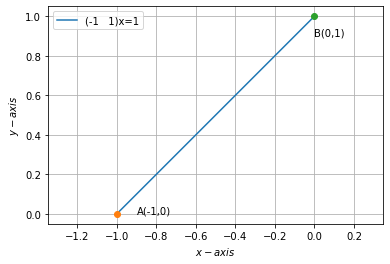
\includegraphics[width=\columnwidth]{Line.png}
\caption{ Plot of a straight line  }
\label{5/1/fig}
\end{figure}


%
\item Find the equation to the straight line cutting off an intercept 2 from the negative direction of the axis of Y and inclined at 30$\degree$ to the X-axis.
\\
\solution

From the given information,
\begin{align}
\vec{m}=\myvec{1\\\frac{1}{\sqrt{3}}},c=-2
\end{align}
The normal vector of the line is
\begin{align}
\vec{n}=\myvec{\frac{-1}{\sqrt{3}}\\1}
\end{align}
Equation of the line in terms of the normal vector is then obtained as
\begin{align}
\vec{n}^{T}\vec{x}&=c
//
\implies \myvec{-1 & \sqrt{3}}\vec{x}=-2\sqrt{3}\label{5/3/fe}
\end{align}
See Fig.         \ref{5/3/fig:Line} 
\begin{figure}[ht!]
       \centering
        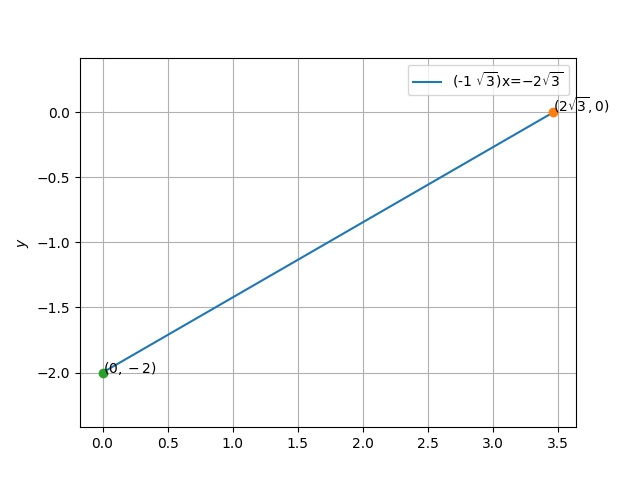
\includegraphics[width =\columnwidth]{fig2.1.png}
        \caption{Plot obtained from python code.We get the required equation.$\myvec{-1 & \sqrt{3}}\vec{x}=-2\sqrt{3}$}
        \label{5/3/fig:Line}
\end{figure}




\item Find the equation to the straight line cutting off an intercept -3 from the axis of y and inclined at an angle $\tan^{-1}\frac{3}{5}$ to the axis of x.
%
\\
\solution

\begin{figure}[!ht]
       \centering
        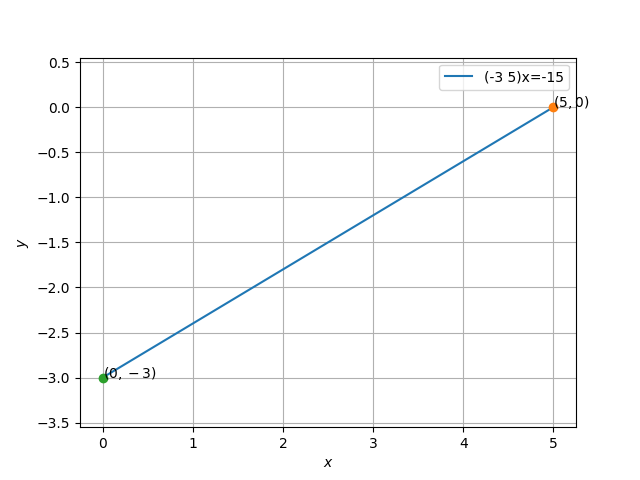
\includegraphics[width =\columnwidth]{line.png}
        \caption{Required plot of the line $\myvec{-3 & 5}\vec{x}=-15$ }
        \label{5/4/fig:Line}
\end{figure}
From the given information, 
\begin{align}
\vec{m}=\myvec{1\\m}\implies\vec{m}=\myvec{1\\\frac{3}{5}},c=-3
\end{align}
Hence, the normal vector of the line is
\begin{align}
\vec{n}=\myvec{\frac{-3}{5}\\1}
\end{align}
Equation of the line is
\begin{align}
\vec{n}^{T}\vec{x}&=c
\\
\implies \myvec{\frac{-3}{5}&1}\vec{x}&=-3
\end{align}
Fig.\ref{5/4/fig:Line} is the plot of the line.





\item Find the equation to the straight line cutting off intercepts 3 and 2 from the axes.
%
\\
\solution
The line passes through the given points
\begin{align}
\vec{x}_{1}=\myvec{3\\0} \text{ and } \vec{x}_{2}=\myvec{0\\2}
\end{align}

Since
\begin{align}
\vec{n}^{T}\vec{x}&=1,
\\
\vec{n}^{T}\myvec{3\\0}&=1\\
\vec{n}^{T}\myvec{0\\2}&=1
\end{align}
%
resulting in the the matrix equation
\begin{align}
\myvec{3 & 0 \\ 0 & 2} \vec{n} = \myvec{1 \\ 1}
\end{align}
%
yielding the augmented matrix
\begin{align}
\myvec{3 &0 & 1\\0 & 2 & 1} 
\end{align}
%
Performing row reduction,
\begin{align}
\myvec{3 &0 & 1\\0 & 2 & 1} 
\\
\xleftrightarrow {R_1\leftarrow \frac{R_1}{3}}\myvec{1 &0 & \frac{1}{3}\\0 & 2 & 1}\\ 
\xleftrightarrow {R_2\leftarrow \frac{R_2}{2}}\myvec{1 &0 & \frac{1}{3}\\0 & 1 & \frac{1}{2}}\\
\label{5/5/eq:line_aug}
\end{align}
%
From \eqref{5/5/eq:line_aug},
\begin{align}
\vec{n} = \frac{1}{6}\myvec{2 \\3}
\end{align}
%
Thus the equation of the desired line is 
\begin{align}
\frac{1}{6}\myvec{2 &3}\vec{x} &= 1
\\
\text{or, } \myvec{2 &3}\vec{x} &= 6
\end{align}
Fig. \ref{5/5/Fig:1} plots the desired line.
\begin{figure}[!ht]
\centering
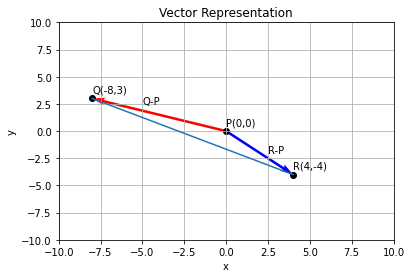
\includegraphics[width=\columnwidth]{image.png}
\caption{Plot obtained from Python code}
\label{5/5/Fig:1}
\end{figure}

%
\item Trace the straight line whose equation is \\
\begin{align}
x + 2y+3 = 0
\end{align}
\\
\solution
The given equation can be expressed as 
\begin{align} \labl{5/11/Eq b}
\myvec{1 & 2}\vec{x} =-3 
\end{align}
Let 
\begin{align}
\vec{x}=\myvec{p\\0}
\end{align}
Substituting in equation \eqref{5/11/Eq b},
\begin{align}
\myvec{1 & 2} \myvec{p\\0} &= -3
\\ \implies p&= -3
\end{align}
Similarly, for 
\begin{align}
\vec{x}=\myvec{0\\q},
\end{align}
substituting in equation \eqref{5/11/Eq b},
\begin{align}
\myvec{1 & 2} \myvec{0\\q} &= -3
\\ \implies q &= \frac{-3}{2}
\end{align}
So, the intercepts of X and Y axes can be obtained as,
\begin{align}
\vec{A}=\myvec{-3\\0} , 
\vec{B}=\myvec{0\\\dfrac{-3}{2}}
\end{align}
%
See Fig. \ref{5/11/Fig:1}.
%
\begin{figure}[h]
\centering
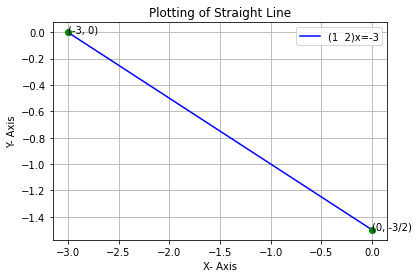
\includegraphics[width=\columnwidth]{solutions/5/11/graph.png}
\caption{Plot obtained from Python code}
\label{5/11/Fig:1}
\end{figure}




\item  Trace the straight line whose equation is
\begin{align}
5x - 7y -9 = 0
\end{align}
%
\\
\solution
%
The given equation can be expressed as 
\begin{align} \label{5/12/Eq b}
\myvec{5 & -7}\vec{x} =9 
\end{align}
Let 
\begin{align}
\vec{x}=\myvec{a\\0}
\end{align}
Substituting in  \eqref{5/12/Eq b},
\begin{align}
\myvec{5 & -7} \myvec{a\\0} &= 9
\\
\implies a & = \frac{9}{5}
\end{align}
Similarly,
\begin{align}
\vec{x}=\myvec{0\\b}
\end{align}
Substituting in  \eqref{5/12/Eq b},
\begin{align}
\myvec{5 & -7} \myvec{0\\b} &= 9
\\ \implies b &= \frac{-9}{7}
\end{align}
So, the intercepts of X and Y axes can be obtained as,
\begin{align}
\vec{A}=\myvec{\dfrac{9}{5}\\0} , 
\vec{B}=\myvec{0\\\dfrac{-9}{7}}
\end{align}
%
See Fig. \ref{5/12/fig}.
%
\begin{figure}[!ht]
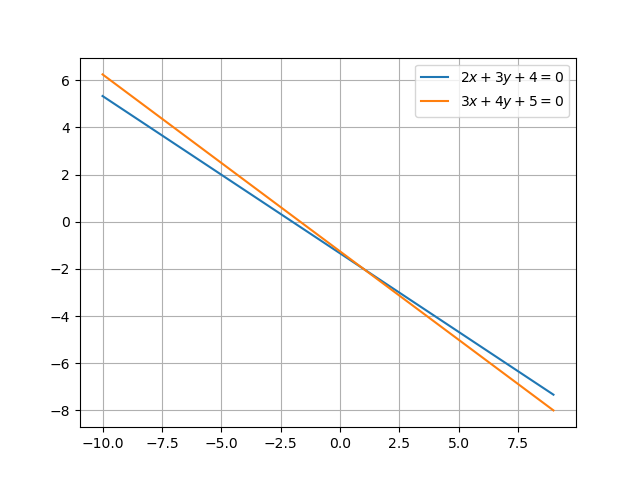
\includegraphics[width=\columnwidth]{Figure_1.png}
\caption{ Plot of the straight line }
\label{5/12/fig}
\end{figure}













\end{enumerate}
